\documentclass[a4paper,12pt]{article}
\usepackage{amsmath,amssymb,amsfonts,amsthm}
\usepackage{tikz}
\usepackage [utf8x] {inputenc}
\usepackage [T2A] {fontenc} 
\usepackage[russian]{babel}
\usepackage{cmap} 
\usepackage{ gensymb }
% Так ссылки в PDF будут активны
\usepackage[unicode]{hyperref}
\usepackage{ textcomp }
\usepackage{indentfirst}
\usepackage[version=3]{mhchem}

% вы сможете вставлять картинки командой \includegraphics[width=0.7\textwidth]{ИМЯ ФАЙЛА}
% получается подключать, как минимум, файлы .pdf, .jpg, .png.
\usepackage{graphicx}
% Если вы хотите явно указать поля:
\usepackage[margin=1in]{geometry}
% Или если вы хотите задать поля менее явно (чем больше DIV, тем больше места под текст):
% \usepackage[DIV=10]{typearea}

\usepackage{fancyhdr}

\newcommand{\bbR}{\mathbb R}%теперь вместо длинной команды \mathbb R (множество вещественных чисел) можно писать короткую запись \bbR. Вместо \bbR вы можете вписать любую строчку букв, которая начинается с '\'.
\newcommand{\eps}{\varepsilon}
\newcommand{\bbN}{\mathbb N}
\newcommand{\dif}{\mathrm{d}}

\newtheorem{Def}{Определение}


\pagestyle{fancy}
\makeatletter % сделать "@" "буквой", а не "спецсимволом" - можно использовать "служебные" команды, содержащие @ в названии
\fancyhead[L]{\footnotesize Квантовая физика}%Это будет написано вверху страницы слева
\fancyhead[R]{\footnotesize ФМХФ МФТИ}
\fancyfoot[L]{\footnotesize \@author}%имя автора будет написано внизу страницы слева
\fancyfoot[R]{\thepage}%номер страницы —- внизу справа
\fancyfoot[C]{}%по центру внизу страницы пусто

\renewcommand{\maketitle}{%
	\noindent{\bfseries\scshape\large\@title\ \mdseries\upshape}\par
	\noindent {\large\itshape\@author}
	\vskip 2ex}
\makeatother
\def\dd#1#2{\frac{\partial#1}{\partial#2}}


\title{2.1 \\ Опыт Франка-Герца}
\author{Егор Берсенев} 
\date{16 февраля 2017 г.}

\begin{document}
	
	\maketitle
	\section{Теоретическое введение
		}
	Опыт Франка-Герца --- простой опыт, подтверждающий дискретность внутренней энергии атома. 
	Разреженный одноатомный газ (He) заполняет трёхэлектродную лампу. Электроны, испускаемые разогретым катодом, ускоряются в постоянном электрическом поле, созданным между катодом и сетчатым анодом лампы. Передвигаясь от катода к аноду, электроны сталкиваются с атомами гелия. Если энергия электрона недостаточна для того, чтобы перевести его в возбужденное состояние (или ионизировать), то возможны только упругие столкновения. По мере увеличения разности потенциалов энергия электронов увеличивается и оказывается достаточной для возбуждения атомов. При таких неупругих столкновениях кинетическая энергия электрона передаётся одному из атомных электронов, вызывая его переход на свободный энергетический уровень (возбуждение) или совсем отрывая его от атома (ионизация).
	
	Третьим электродом лампы является коллектор. Между ним и анодом поддерживается небольшое задерживающее напряжение. Ток коллектора измеряется микроамперметром.
	При увеличении потенциала анода ток в лампе вначале растет, а когда энергия электронов становится достаточной для возбуждения атомов, ток коллектора резко уменьшается, так как электроны почти полностью теряют свою энергию при неупругих соударениях с атомами. При дальнейшем увеличении потенциала анода ток коллектора вновь возрастает. Следующее замедление роста тока происходит в момент, когда часть электронов неупруго сталкивается с атомами два раза: первый раз посередине пути, второй -- у анода. Таким образом, на кривой зависимости тока коллектора от напряжения анода имеется ряд максимумов и минимумов, отстоящих друг от друга на равные расстояния $\Delta V$, равные энергии первого возбуждённого состояния.
	
	Теория, описывающая дискретность энергетических уровней атома He довольно сложная в плане вычислений, а концептуально всё сводится к решению уравнения Шрёдингера.
	
	Гамильтониан системы выглядит следующим образом
	
	\begin{equation}
		\hat{H}=-\frac{\hbar^2}{2m}\Delta_1-\frac{\hbar^2}{2m}\Delta_2-\frac{Ze^2}{4\pi\varepsilon r_1}-\frac{Ze^2}{4\pi\varepsilon r_2}+\frac{e^2}{4\pi\varepsilon r_{12}}
	\end{equation}
	
	Решить требуется стационарное уравнение Шрёдингера
	
	\begin{equation}
		\hat{H}\Psi({\bf r}_1,\,{\bf r}_2)=E\Psi({\bf r}_1,\,{\bf r}_2)
	\end{equation}
	
	Гамильтониан можно переписать в виде
	
	\begin{equation}
		\hat{H}=\hat{H}_1+\hat{H}_2+V_{12},
	\end{equation}
	
	где $V_{12}$ описывает взаимодействие электронов, которым традиционно пренебрегают, разделяют переменные и решают одноэлектронные уравнения Шрёдингера, получая приблизительную волновую функцию, затем используя соображения о принципе запрета Паули и т.д. учитывают спин электронов и делают поправки на их взаимодействие. Описание этой процедуры выходит за рамки работы, поэтому нет нужды описывать её подробно.
	
	\section{Экспериментальная часть}
		Сначала исследуем ВАХ в динамическом режиме. Для трех значений задерживающего напряжения получим осциллограммы. Важно заметить, что развертка осуществляется справа налево. Цена деления осциллографа $5V$.
		
		\begin{figure}[h!]
			\begin{center}
				\begin{minipage}{0.3\textwidth}
					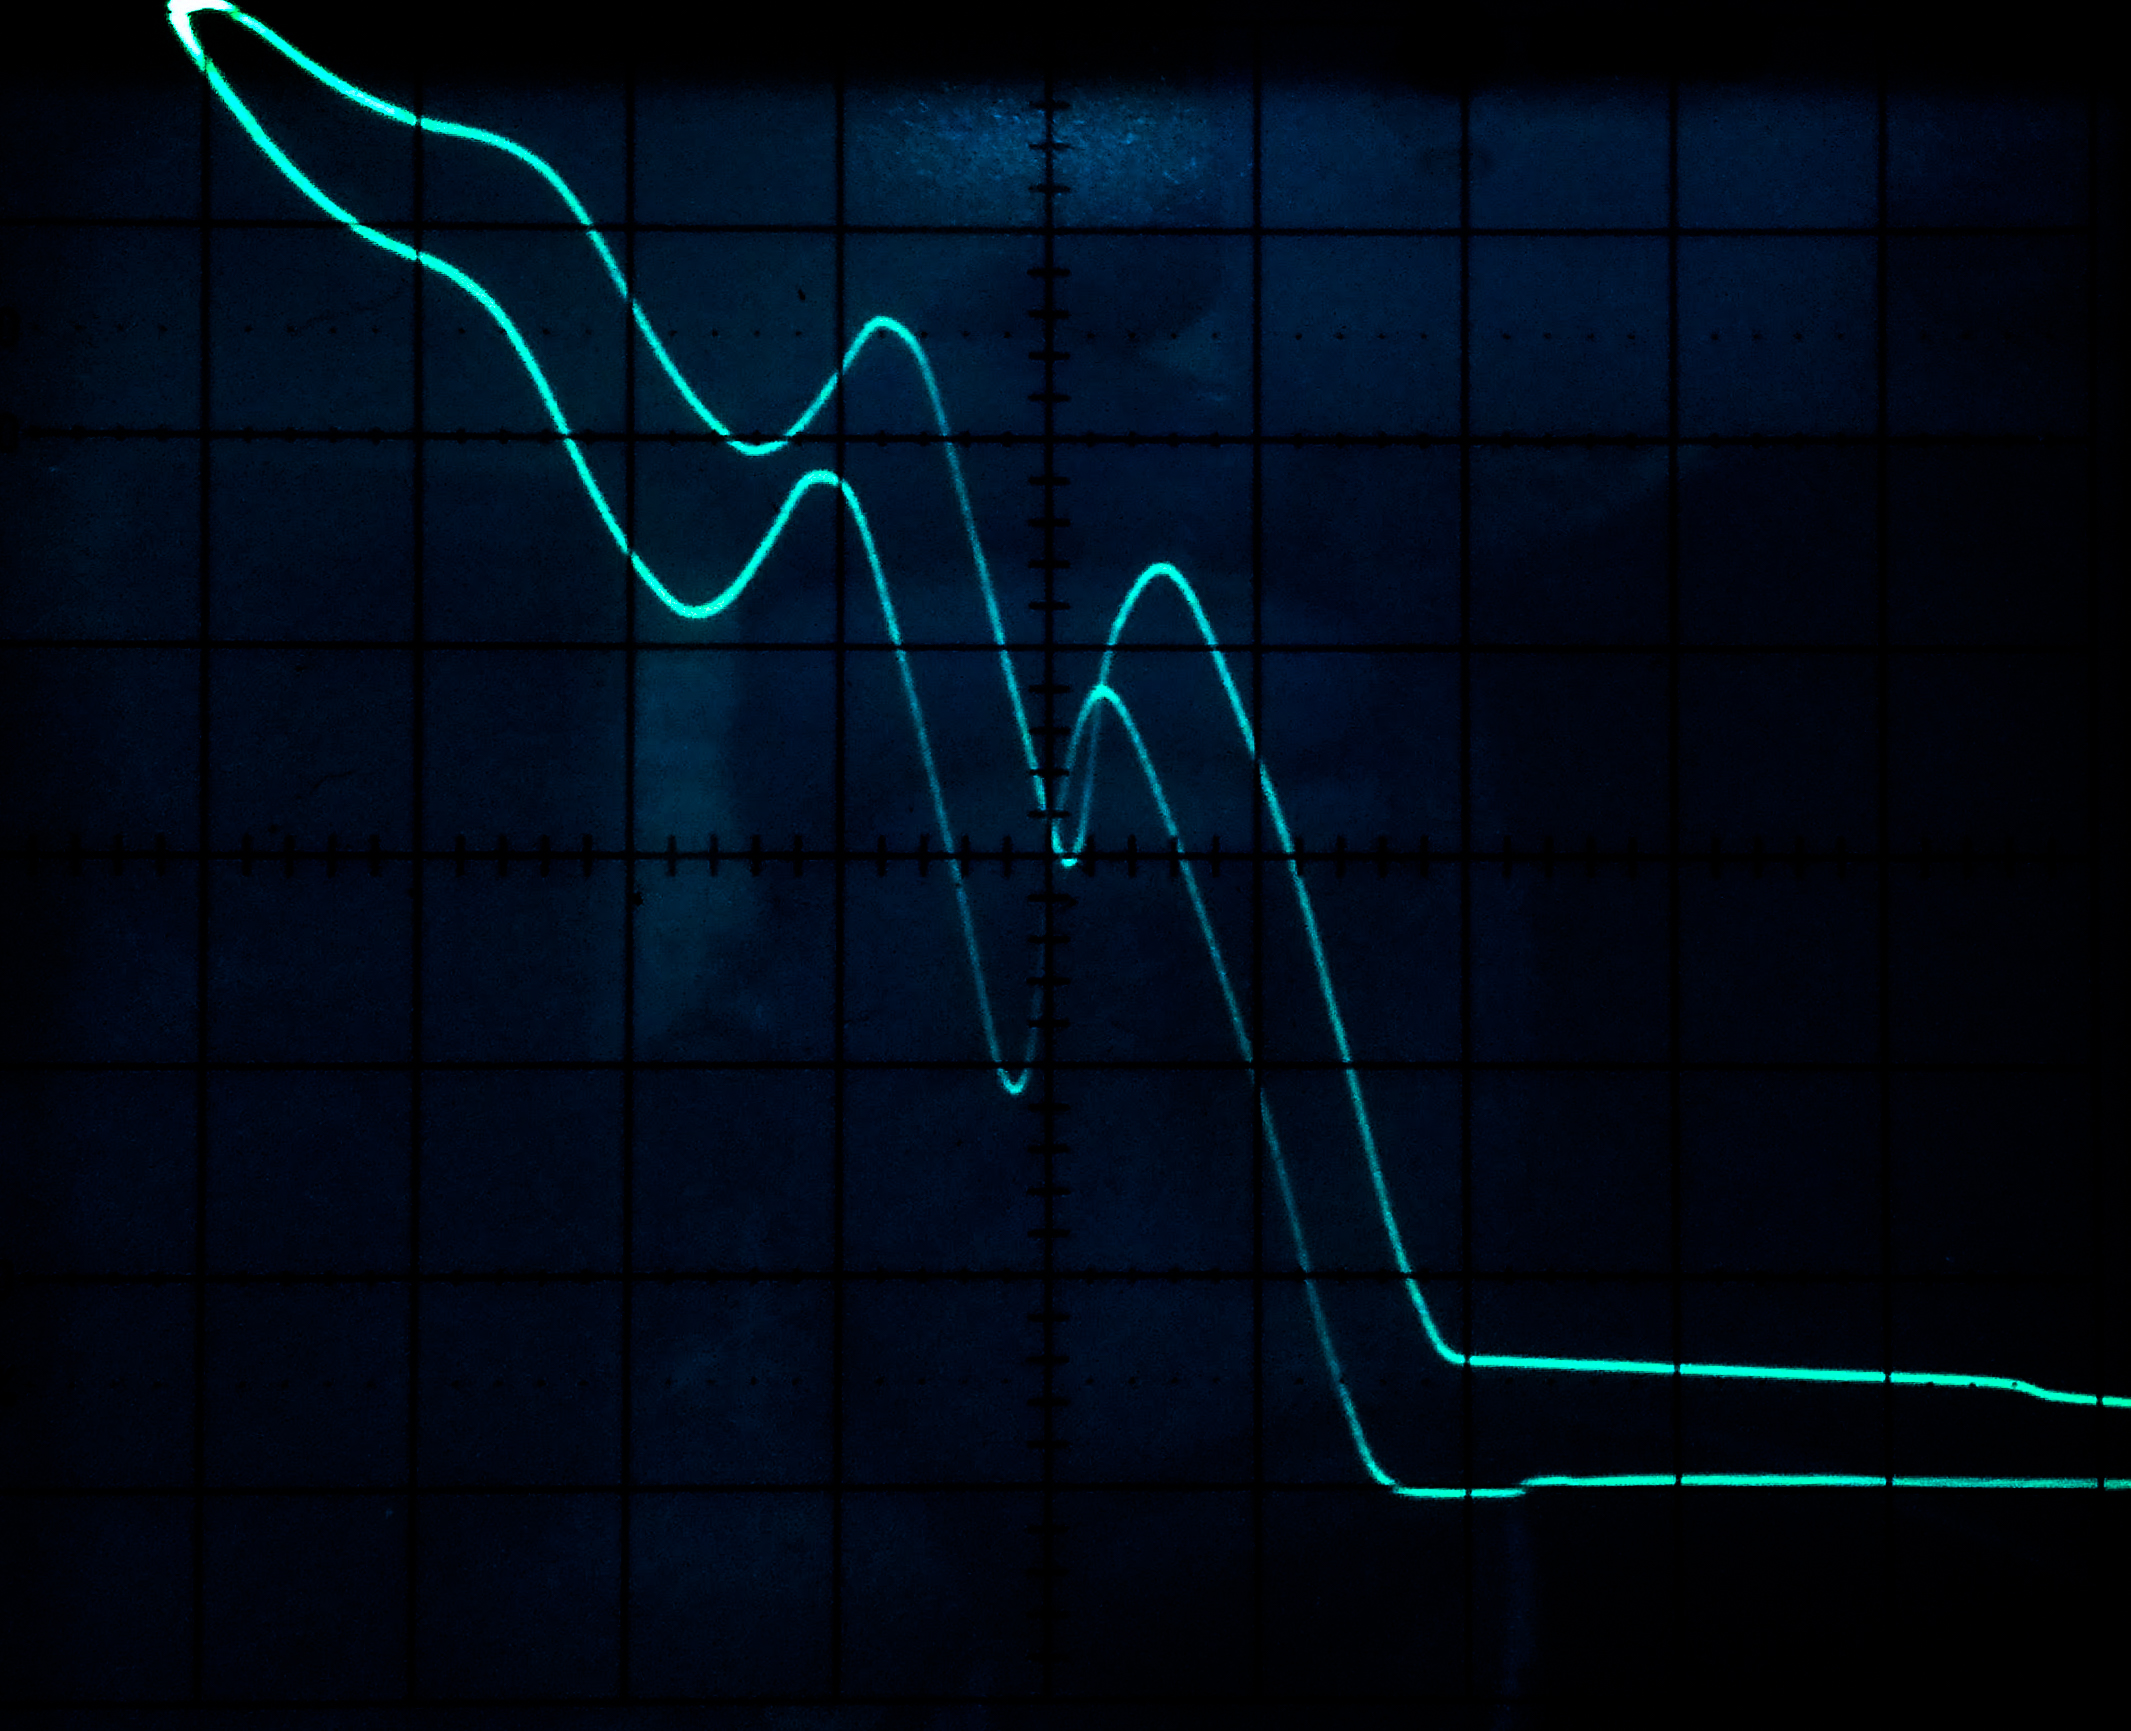
\includegraphics[width=\textwidth]{4}
					\caption{$U = 4V$}
					\end{minipage}
					\hfill
					\begin{minipage}{0.3\textwidth}
						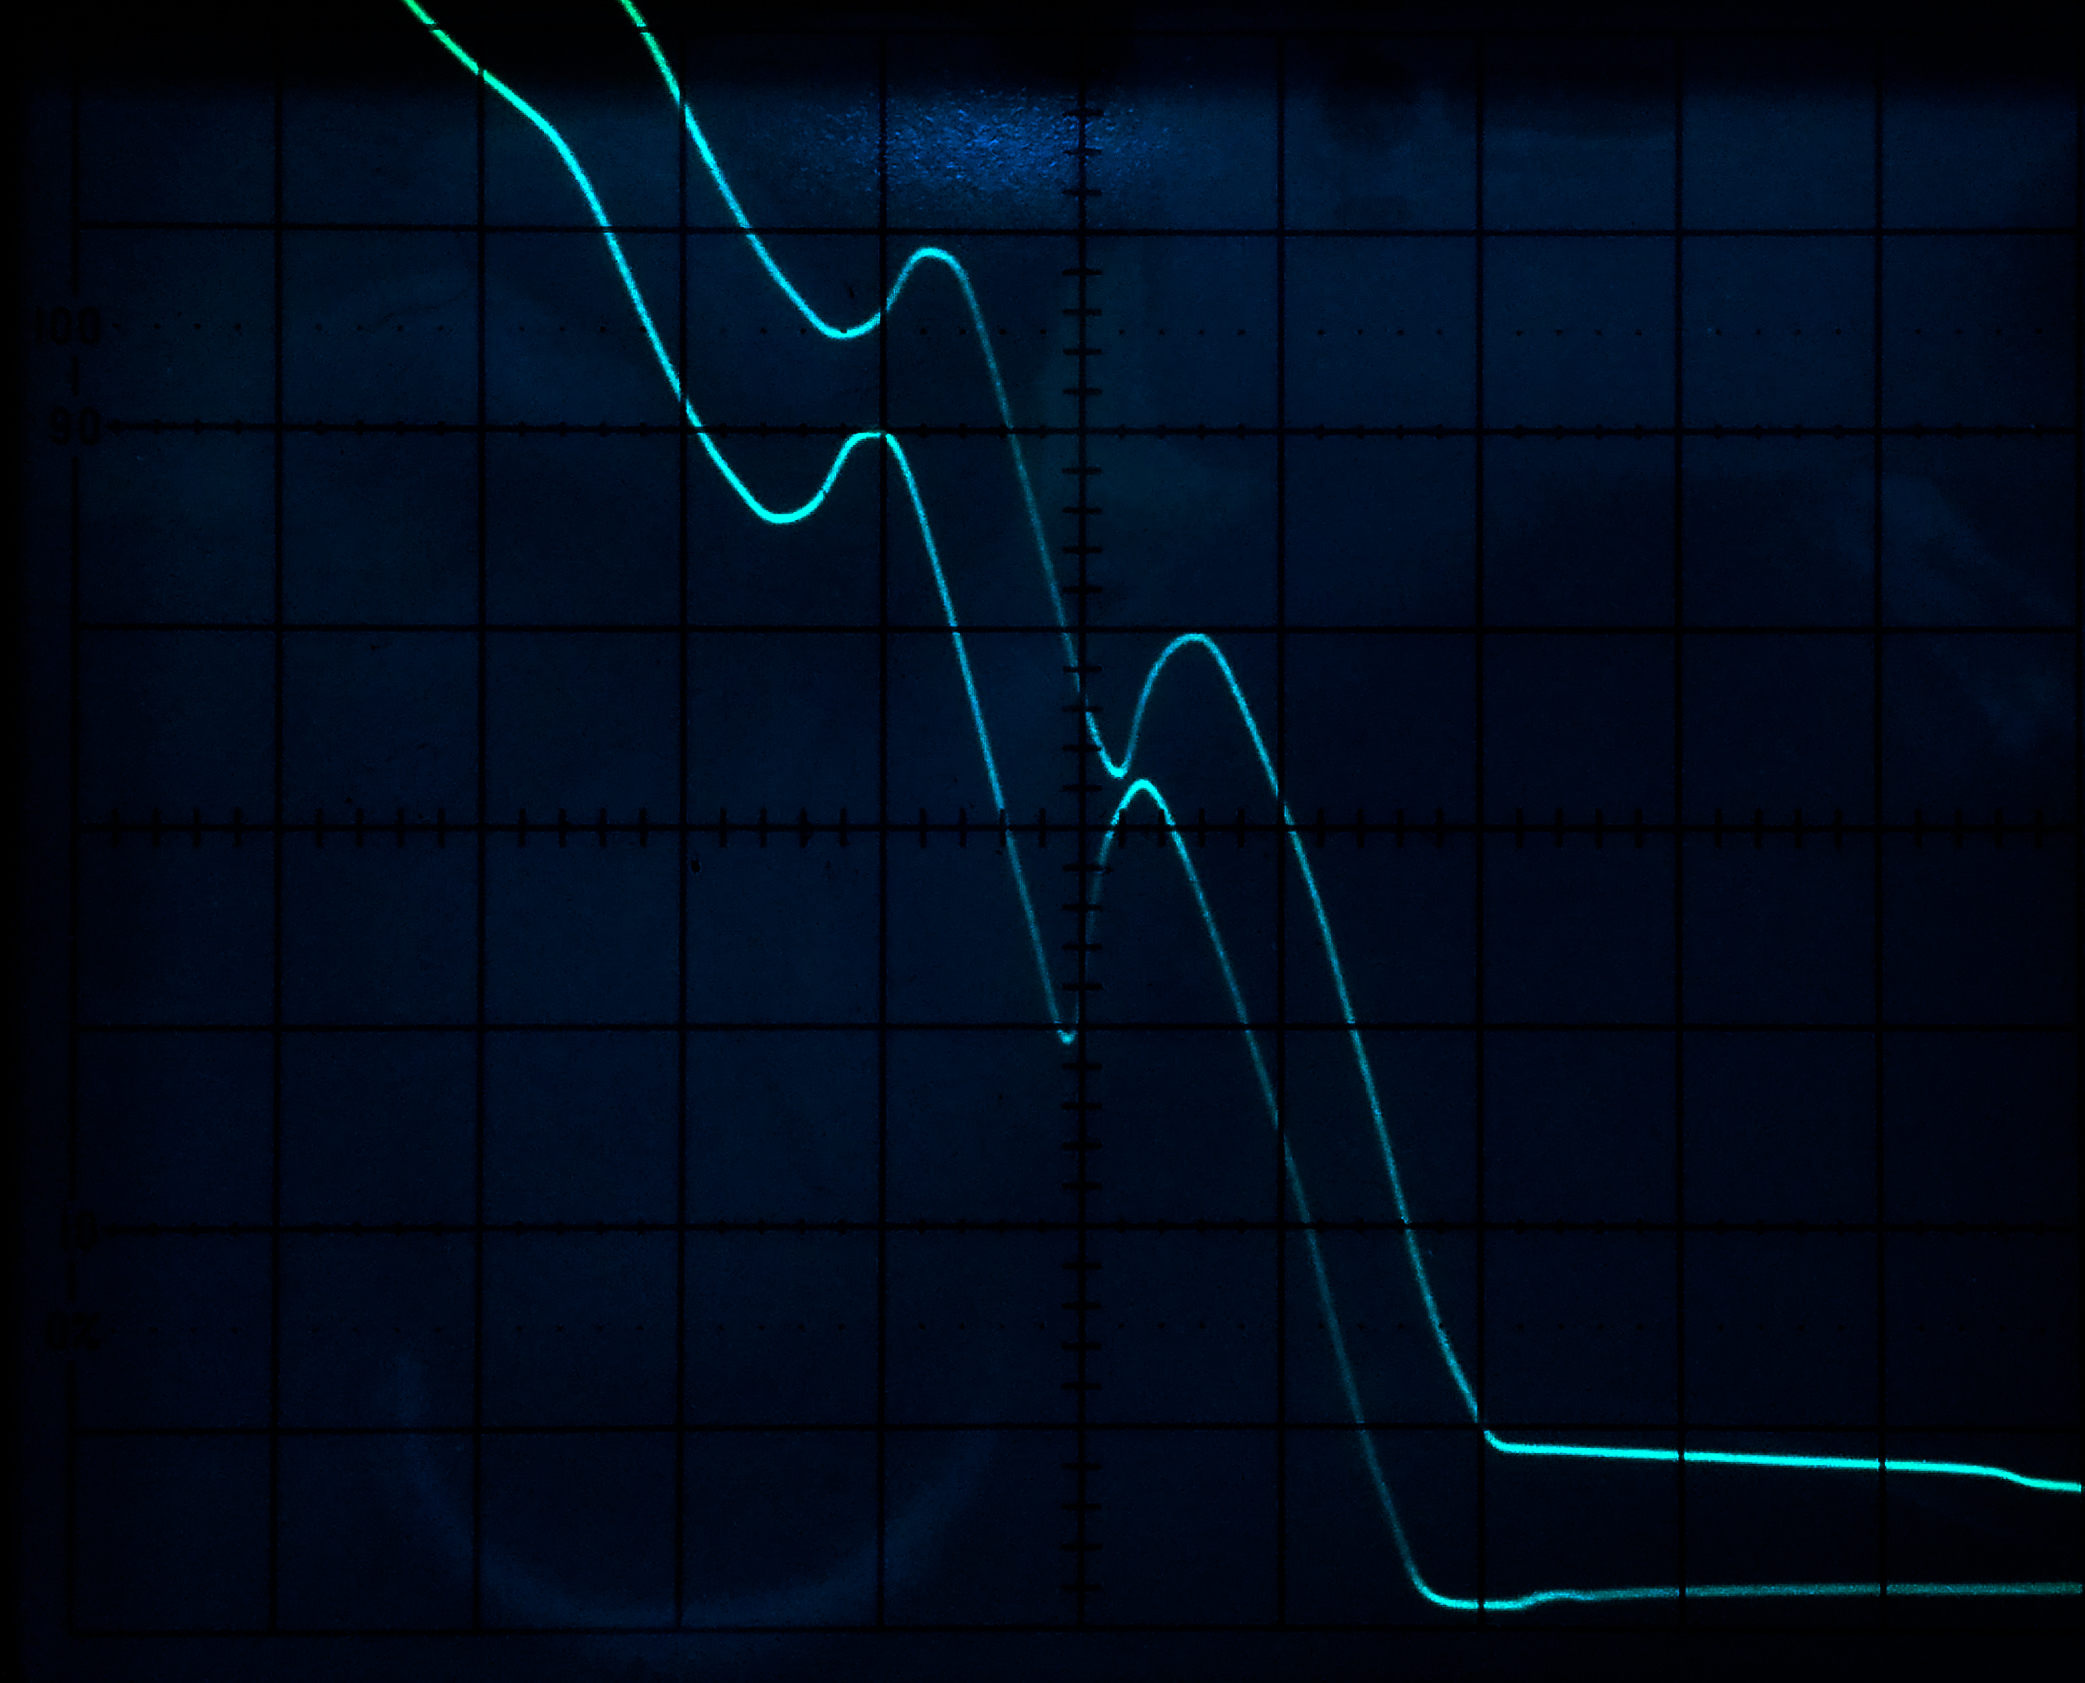
\includegraphics[width=\textwidth]{6}
						\caption{$U = 6V$}
					\end{minipage}
						\hfill
					\begin{minipage}{0.3\textwidth}
						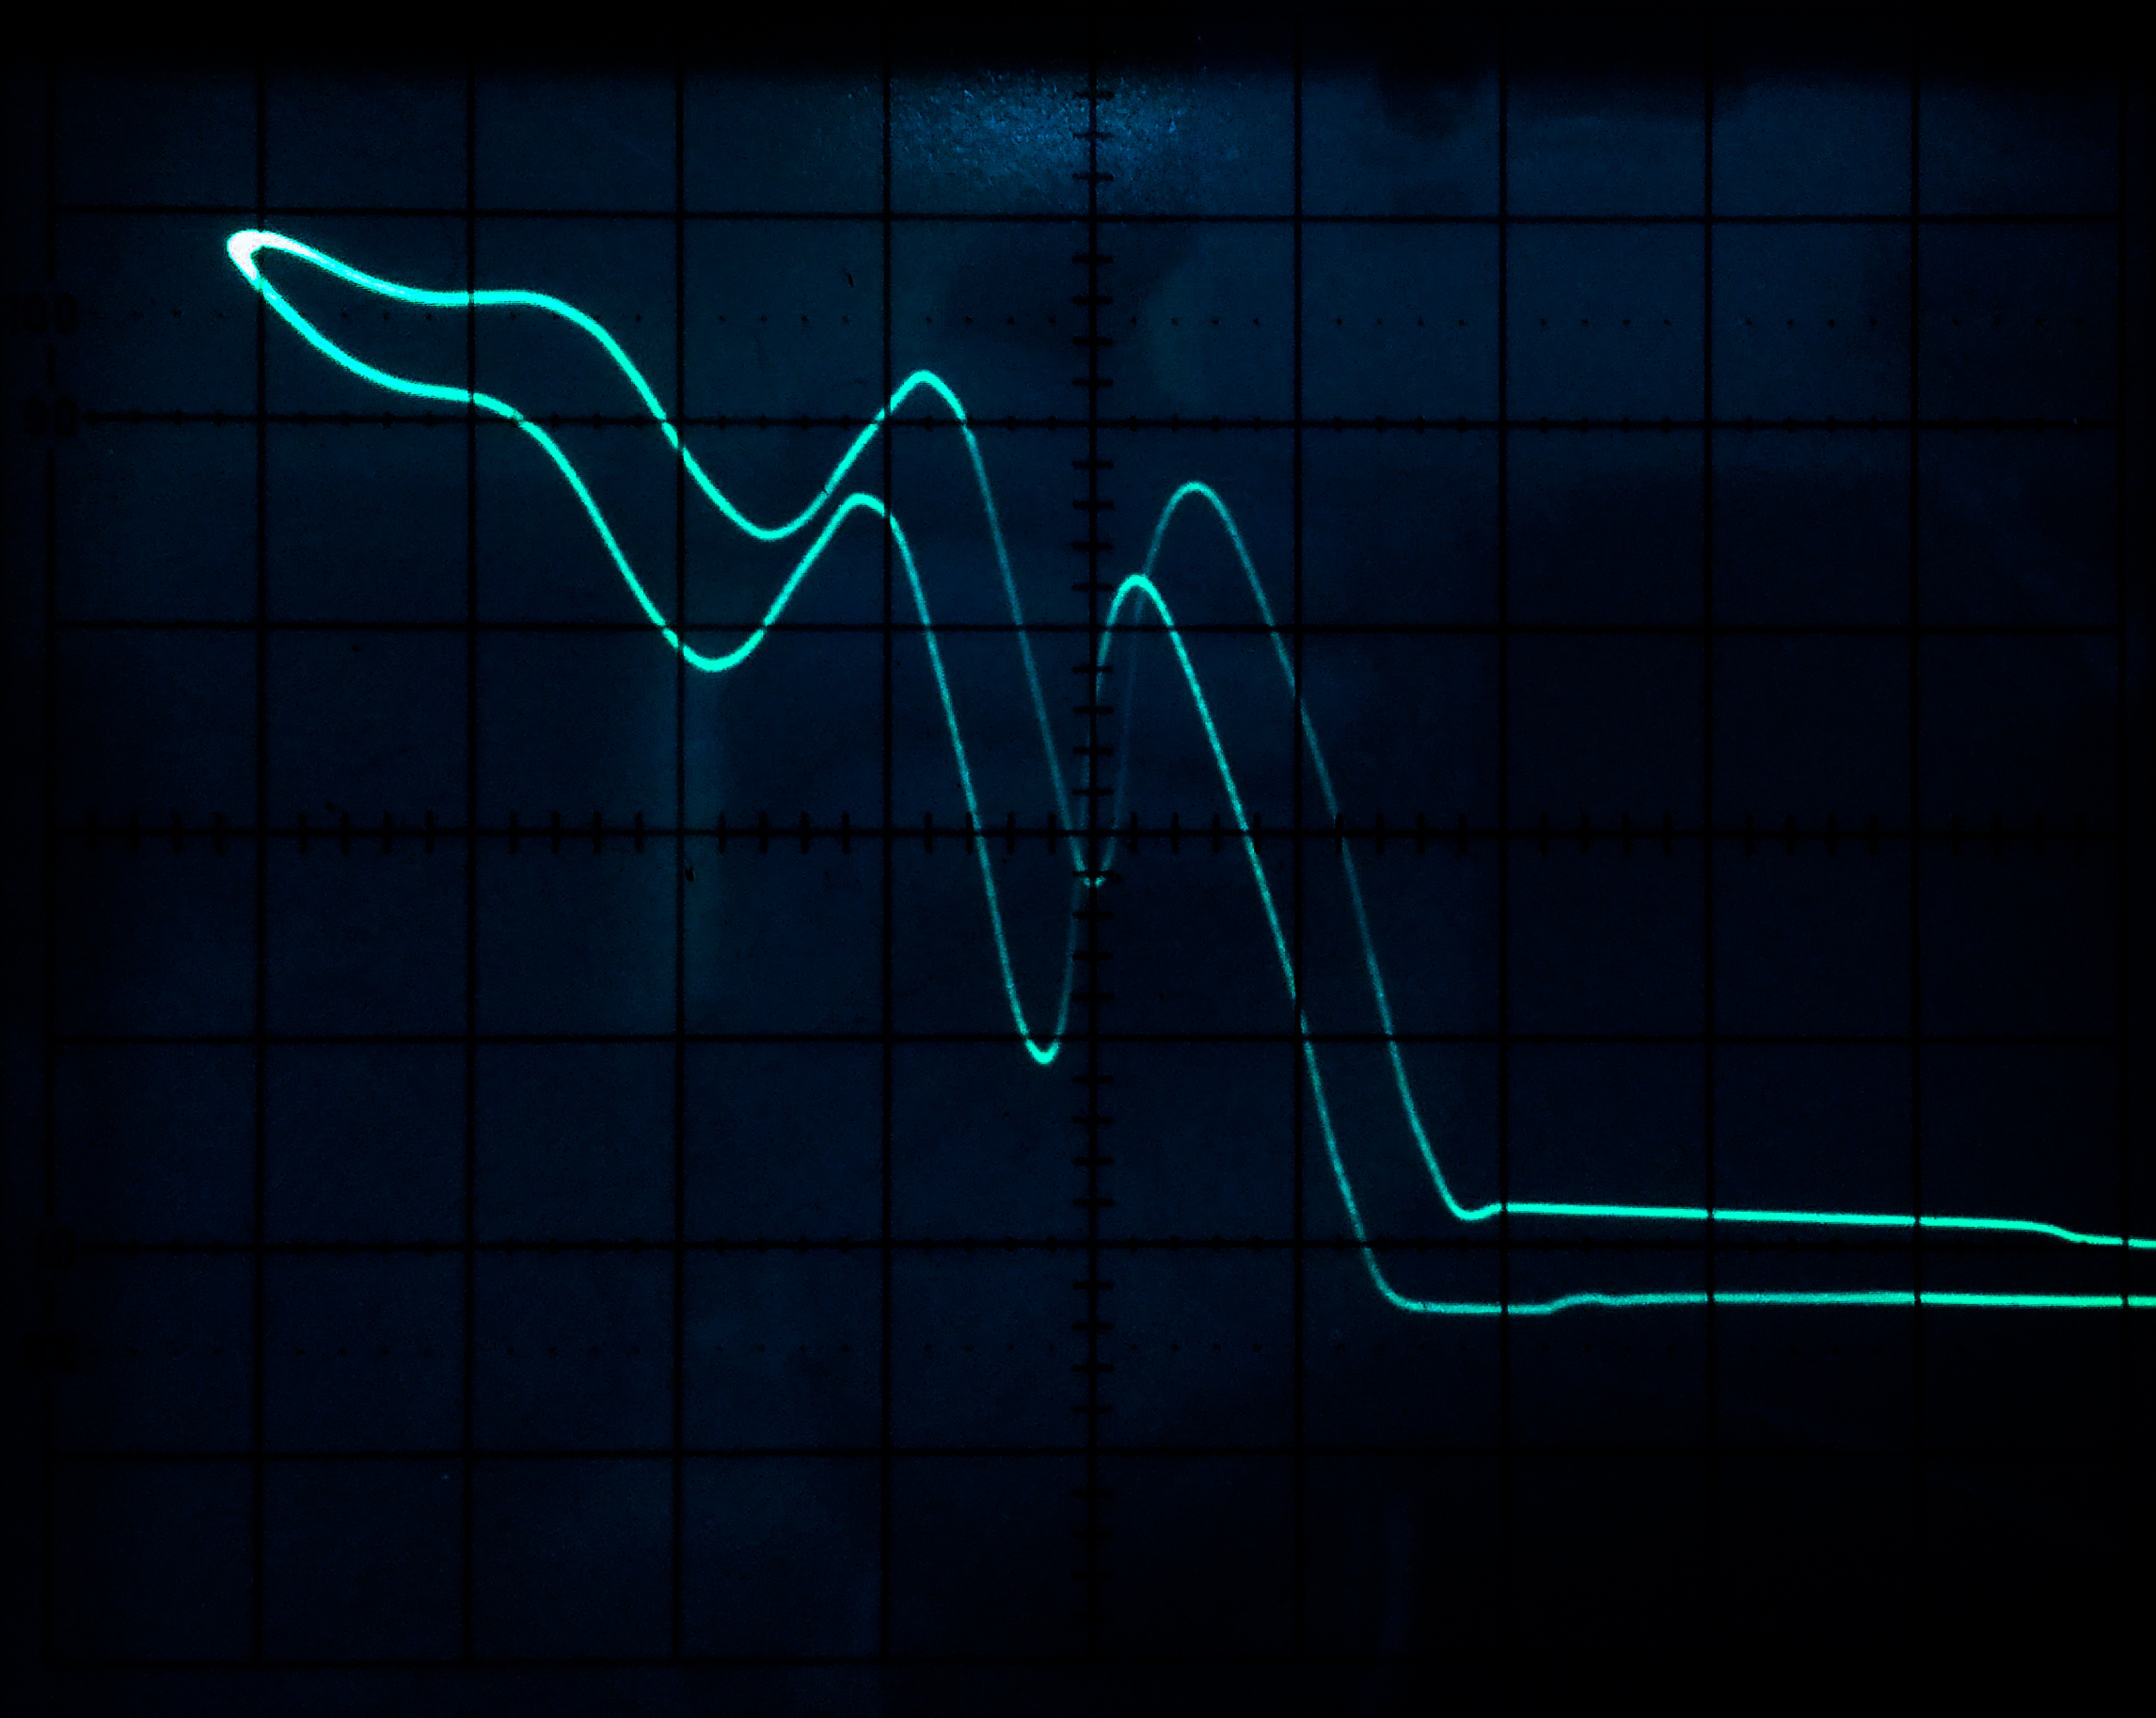
\includegraphics[width=\textwidth]{8}
						\caption{$U = 8V$}
					\end{minipage}
			\end{center}
		\end{figure}
		
		Затем, исследуем ВАХ более подробно, перейдя в статический режим.
		\begin{figure}[h!]
			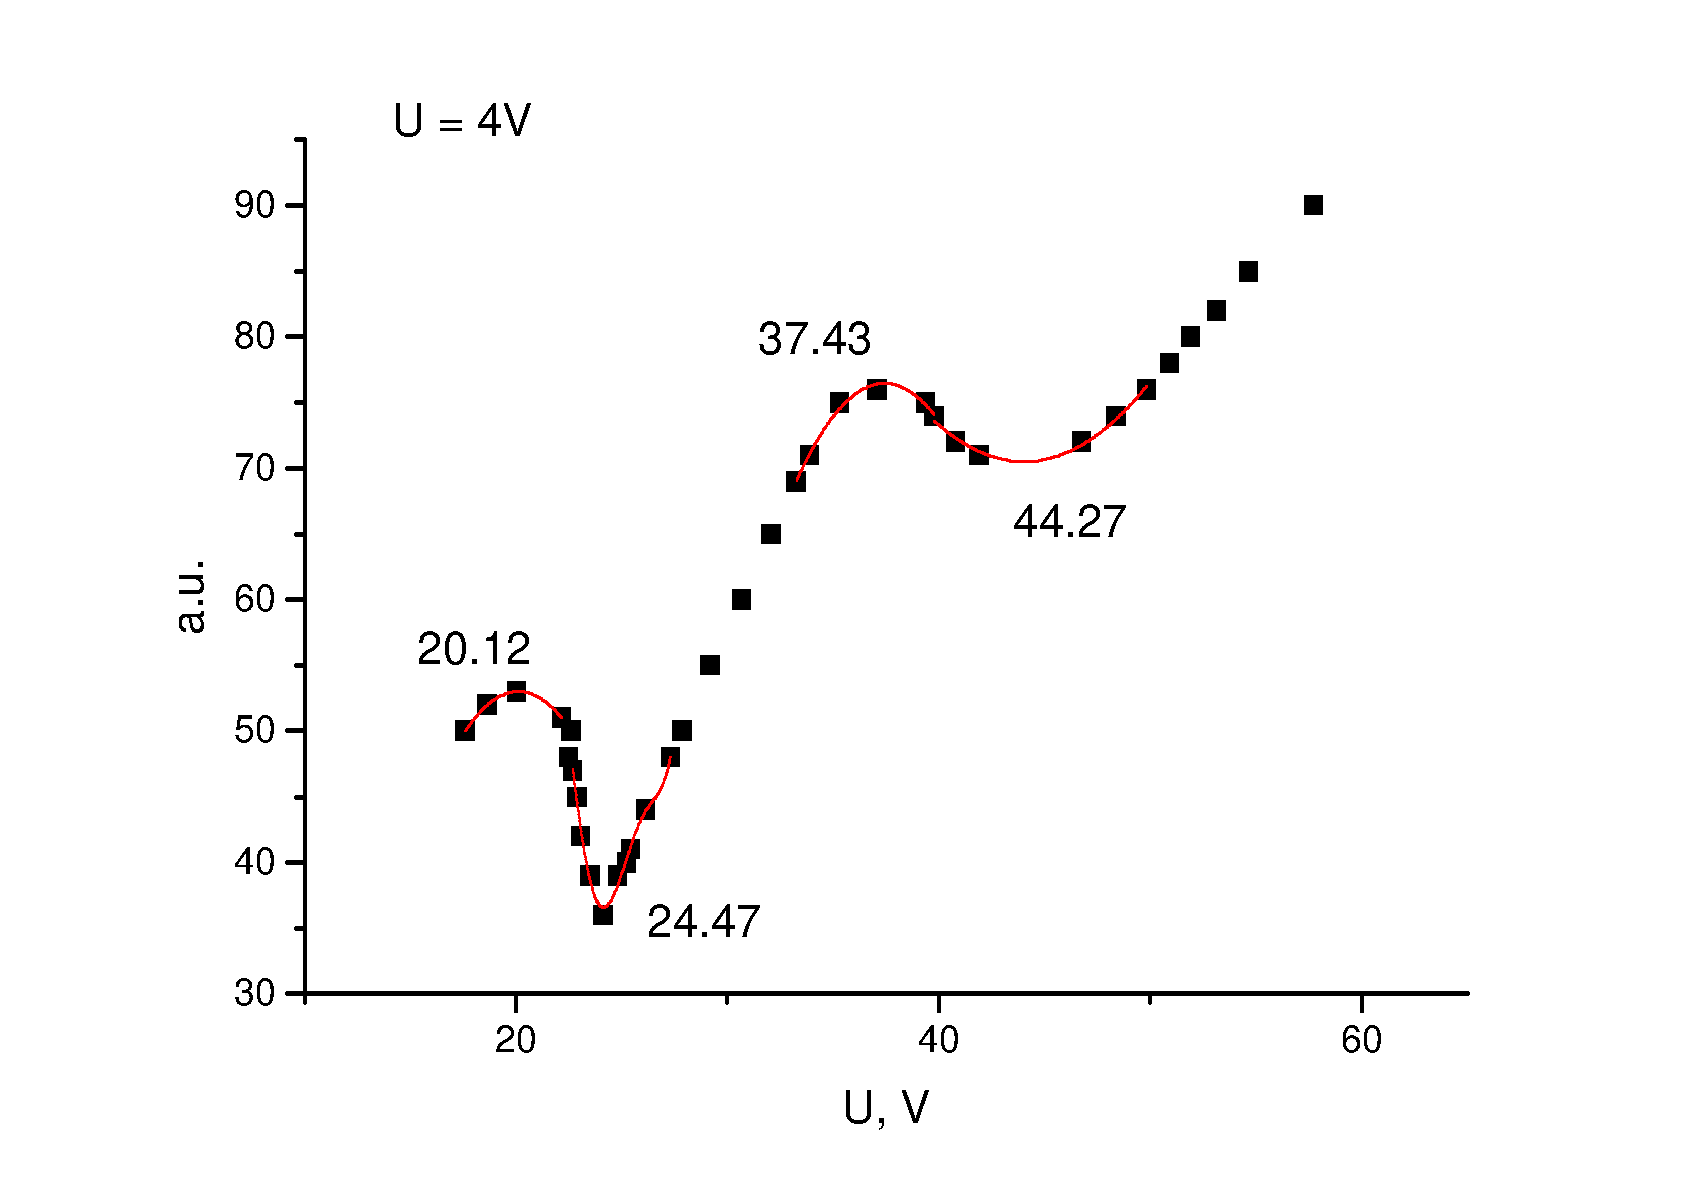
\includegraphics[width=0.95\linewidth]{4V}
			\caption{$U = 4V$}
		\end{figure}
		
		\begin{figure}[h!]
			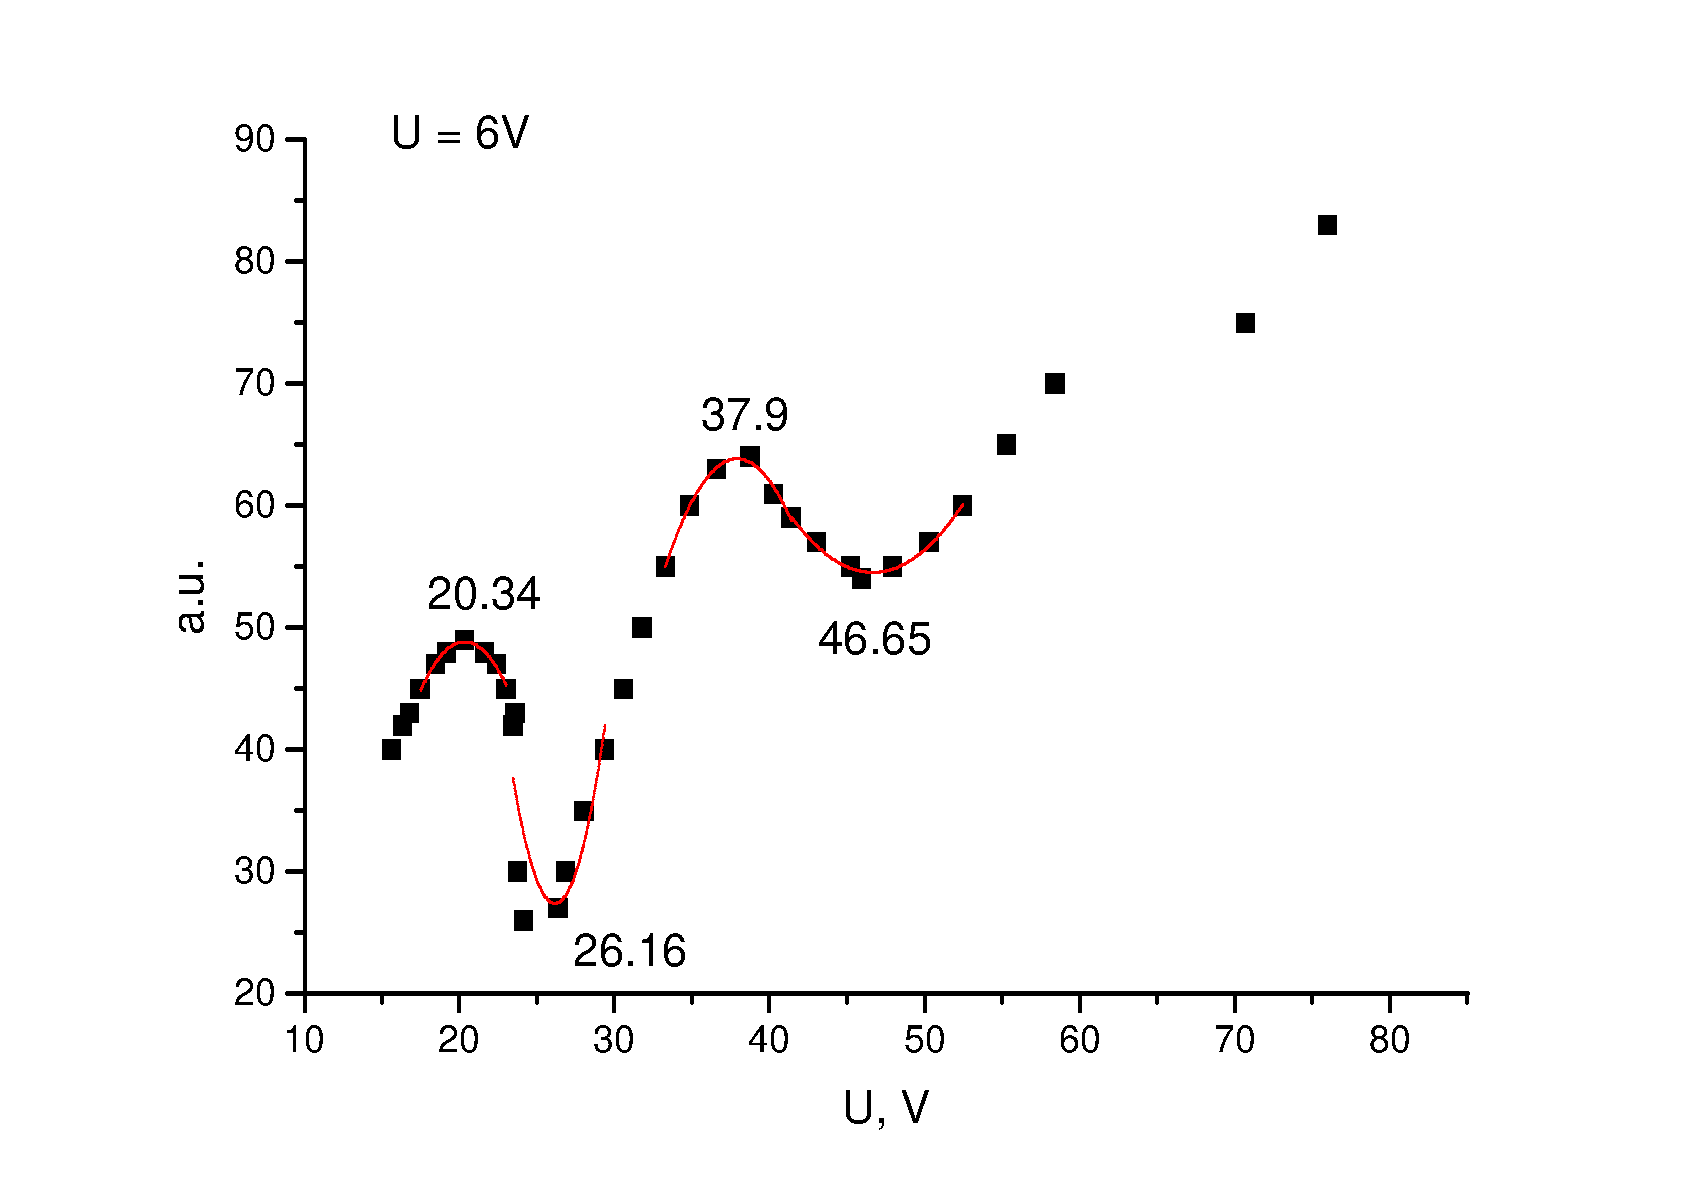
\includegraphics[width=0.95\linewidth]{6V}
			\caption{$U = 6V$}
		\end{figure}
		
		\begin{figure}[h!]
			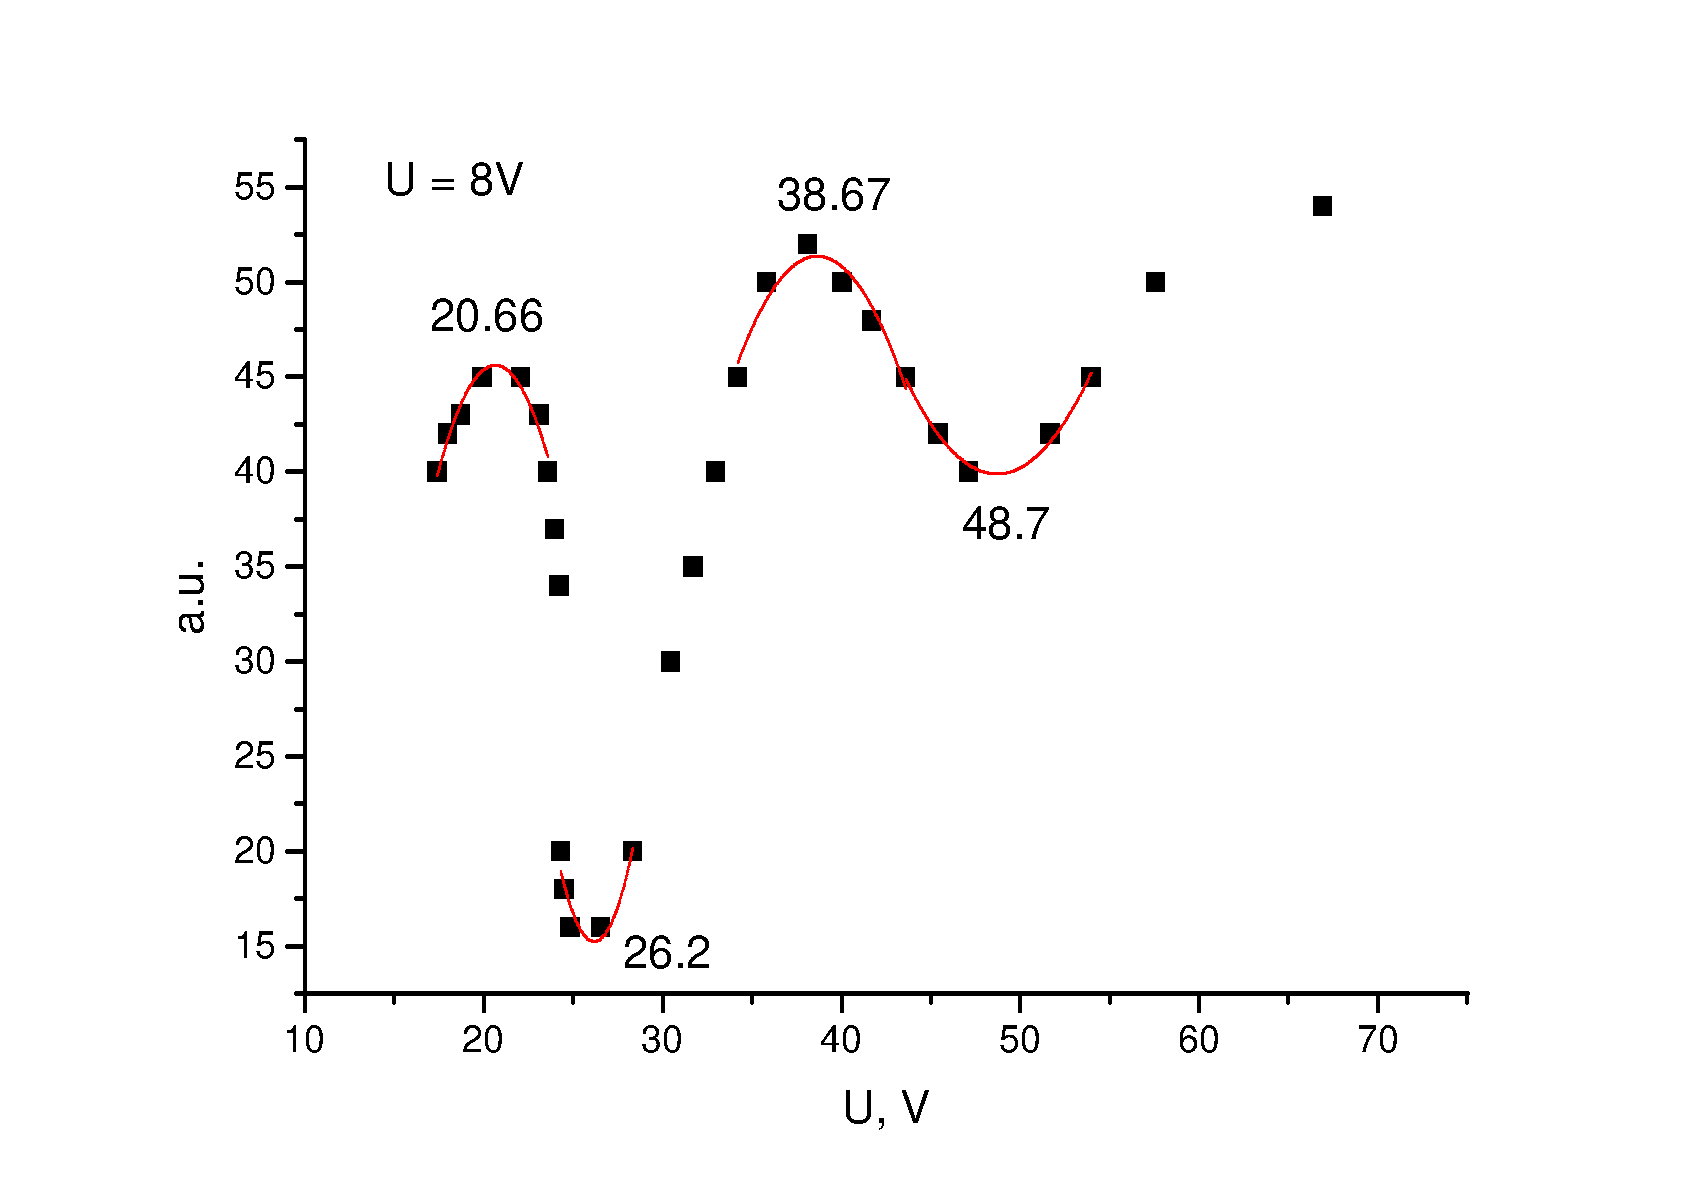
\includegraphics[width=0.95\linewidth]{8V}
			\caption{$U = 8V$}
		\end{figure}
		
		\begin{table}[h!]
			\centering
			\caption{Статический режим}
			\label{my-label}
			\begin{tabular}{|c|c|c|c|c|c|c|}
				\hline
				U, V & $V_{max1}$ & $V_{max2}$ & $\Delta V_{max}$ & $V_{min1}$ & $V_{min2}$ & $\Delta V_{min}$ \\ \hline
				4    & $20.12 \pm 0.5$      & $37.43 \pm 0.5$       & $17.31 \pm 0.7$            & $24.47 \pm 0.5$     & $44.27 \pm 0.5$      & $19.8 \pm 0.7$           \\ \hline
				6    & $20.34 \pm 0.5$      & $37.9 \pm 0.5$     & $17.56 \pm 0.7$           & $26.16 \pm 0.5$     & $46.65 \pm 0.5$      & $20.49 \pm 0.7$            \\ \hline
				8    & $20.66 \pm 0.5$     & $38.67 \pm 0.5$     & $18.01 \pm 0.7$           & $26.2 \pm 0.5$     & $48.7 \pm 0.5$       & $22.5 \pm 0.7$           \\ \hline
			\end{tabular}
		\end{table}
		
	
		\begin{table}[h!]
			\centering
			\caption{Табличные значения для атома гелия}
			\label{table3}
			\begin{tabular}{|c|c|}
				\hline
				$E_I$                                  & 24,47 эВ \\ \hline
				$E_1$ & 19,82 эВ \\ \hline
			\end{tabular}
		\end{table}
		
		\section{Обсуждение результатов и выводы}
			Проделанная работа позволяет убедится в дискретности энергетических уровней в атоме гелия. Снятие вольт-амперной характеристики в динамическом режиме позволяет наглядно увидеть структуру энергетических уровней. Статический режим же нужен для более точного измерения энергии возбуждения атома. Эксперимент показал, что измеренная нами энергия атома близка к табличной(сходится по порядку величины).
			
\end{document}


